%sage: G = Graph([[1,3],[2,3],[3,4]])                                                                                                                                                                      
%sage: GP = GraphicalPolytopes(G)                                                                                                                                                                          
%sage: CP = GP.chunk_polytope(tuple([3]), tuple([3]), weights=GP.standard_weights(), essential=True)                                                                                                       
%sage: to_tikz(CP, nb=True)                                                                                                                                                                                

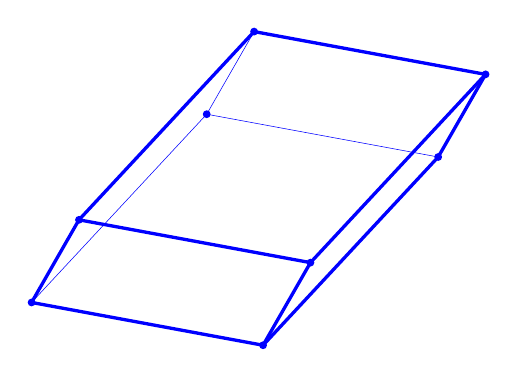
\begin{tikzpicture}%
	[x={(-0.366215cm, -0.789554cm)},
	y={(0.235950cm, -0.590693cm)},
	z={(0.900119cm, -0.166391cm)},
	scale=.5,
	back/.style={very thin},
	edge/.style={color=blue, very thick},
	facet/.style={fill=blue,fill opacity=0},
	vertex/.style={inner sep=1pt,circle,fill=blue,thick},
	baseline=0]

%% Coordinate of the vertices:
%%
\coordinate (-3.33333, -4.71405, 1.63299) at (-3.33333, -4.71405, 1.63299);
\coordinate (-3.33333, -4.71405, 8.16497) at (-3.33333, -4.71405, 8.16497);
\coordinate (-3.33333, -0.47140, -0.81650) at (-3.33333, -0.47140, -0.81650);
\coordinate (-3.33333, -0.47140, 5.71548) at (-3.33333, -0.47140, 5.71548);
\coordinate (2.00000, -2.82843, -1.63299) at (2.00000, -2.82843, -1.63299);
\coordinate (2.00000, -2.82843, 4.89898) at (2.00000, -2.82843, 4.89898);
\coordinate (2.00000, 1.41421, -4.08248) at (2.00000, 1.41421, -4.08248);
\coordinate (2.00000, 1.41421, 2.44949) at (2.00000, 1.41421, 2.44949);
%%
%%
%% Drawing edges in the back
%%
\draw[edge,back] (-3.33333, -4.71405, 1.63299) -- (-3.33333, -0.47140, -0.81650);
\draw[edge,back] (-3.33333, -0.47140, -0.81650) -- (-3.33333, -0.47140, 5.71548);
\draw[edge,back] (-3.33333, -0.47140, -0.81650) -- (2.00000, 1.41421, -4.08248);
%%
%%
%% Drawing vertices in the back
%%
\node[vertex] at (-3.33333, -0.47140, -0.81650)     {};
%%
%%
%% Drawing the facets
%%
\fill[facet] (2.00000, -2.82843, 4.89898) -- (-3.33333, -4.71405, 8.16497) -- (-3.33333, -4.71405, 1.63299) -- (2.00000, -2.82843, -1.63299) -- cycle {};
\fill[facet] (2.00000, 1.41421, 2.44949) -- (-3.33333, -0.47140, 5.71548) -- (-3.33333, -4.71405, 8.16497) -- (2.00000, -2.82843, 4.89898) -- cycle {};
\fill[facet] (2.00000, 1.41421, 2.44949) -- (2.00000, -2.82843, 4.89898) -- (2.00000, -2.82843, -1.63299) -- (2.00000, 1.41421, -4.08248) -- cycle {};
%%
%%
%% Drawing edges in the front
%%
\draw[edge] (-3.33333, -4.71405, 1.63299) -- (-3.33333, -4.71405, 8.16497);
\draw[edge] (-3.33333, -4.71405, 1.63299) -- (2.00000, -2.82843, -1.63299);
\draw[edge] (-3.33333, -4.71405, 8.16497) -- (-3.33333, -0.47140, 5.71548);
\draw[edge] (-3.33333, -4.71405, 8.16497) -- (2.00000, -2.82843, 4.89898);
\draw[edge] (-3.33333, -0.47140, 5.71548) -- (2.00000, 1.41421, 2.44949);
\draw[edge] (2.00000, -2.82843, -1.63299) -- (2.00000, -2.82843, 4.89898);
\draw[edge] (2.00000, -2.82843, -1.63299) -- (2.00000, 1.41421, -4.08248);
\draw[edge] (2.00000, -2.82843, 4.89898) -- (2.00000, 1.41421, 2.44949);
\draw[edge] (2.00000, 1.41421, -4.08248) -- (2.00000, 1.41421, 2.44949);
%%
%%
%% Drawing the vertices in the front
%%
\node[vertex] at (-3.33333, -4.71405, 1.63299)     {};
\node[vertex] at (-3.33333, -4.71405, 8.16497)     {};
\node[vertex] at (-3.33333, -0.47140, 5.71548)     {};
\node[vertex] at (2.00000, -2.82843, -1.63299)     {};
\node[vertex] at (2.00000, -2.82843, 4.89898)     {};
\node[vertex] at (2.00000, 1.41421, -4.08248)     {};
\node[vertex] at (2.00000, 1.41421, 2.44949)     {};
%%
%%
\end{tikzpicture}